\capitulo{6}{Trabajos relacionados}

Existe una literatura variada sobre técnicas para la rehabilitación de pacientes de la enfermedad del \textit{Parkinson} así como de aproximaciones para el análisis de vídeo en tiempo real. En este capítulo se expondrán algunos de los más relevantes.

\section{Literatura científica relacionada}

En el año 2019, Linares-del Rey \textit{et. al.}~\cite{linares2019aplicaciones} realizaron un meta-análisis sobre un total de veintiséis artículos de aplicaciones móviles para pacientes de \textit{Parkinson}. Se consideraron artículos en castellano y en inglés entre los años 2011 y 2016. Además se analizaron ciento tres aplicaciones móviles que estuviesen en los principales \textit{marketplaces}: \textit{Google Play}, \textit{App Store} y \textit{Windows Store}.

El conjunto de estudios abarcaba a un total de cuatrocientos veinte pacientes y docientos treinta y dos personas sanas, estos como grupo de control en los artículos que los incluían. 

Para valorar la calidad metodológica de estos artículos se utilizó la escala JADAD~\cite{jadad1996assessing} basada en si existe o no aleatorización de los participantes, y se describe el método, si se hace un estudio de doble ciego, y se describe el método llevado para ello, y si se describen adecuadamente las pérdidas. Se suele tomar como valor mínimo aceptable una puntación de~tres.

Entre el total de artículos revisados el único con una puntuación aceptable fue el sistema \textit{CuPid}~\cite{ginis2016feasibility} con un total de cuarenta participantes. La aplicación que presenta evaluaba la mejora de la calidad de vida del paciente según mejorasen su equilibrio, marcha y resistencia. Sin embargo, esta aplicación requería de uso de sensores externos al dispositivo móvil para poder evaluar la aplicación.

Respecto a las aplicaciones, al no tener artículos asociados (ya que de tenerlos se habrían analizado en el primer conjunto) no se podían evaluar siguiendo la misma escala. Sin embargo, algunas aplicaciones de las que se analizaron ya estaban incluidas en otras revisiones similares a las de Linares-del Rey \textit{et. al.}

La conclusión de los autores fue que debido a la baja calidad metodológica y la poca cantidad de estudios realizados, no se podía recomendar un uso generalizado de las aplicaciones, es decir, sigue haciendo falta la supervisión de terapeutas especializados que puedan dirigir y ayudar a la mejora de la calidad de vida de los pacientes.

\section{Aproximaciones en problemas similares}

El arquitecto de software Amit Baghel prensentó en 2016 una aproximación en Java para procesar vídeo utilizando \textit{Kafka} junto a \textit{Spark}~\cite{amit2017kafka}.

El objetivo de su trabajo era la creación de un detector de movimiento que combinase en una misma cola de \textit{Kafka} diferentes fuentes de vídeo y las procesase utilizando \textit{OpenCV} junto a \textit{Spark Streaming} y comparar cada \textit{frame} con el anterior y así detectar los objetos que se hubiesen movido.

\begin{figure}[h]
	\centering
	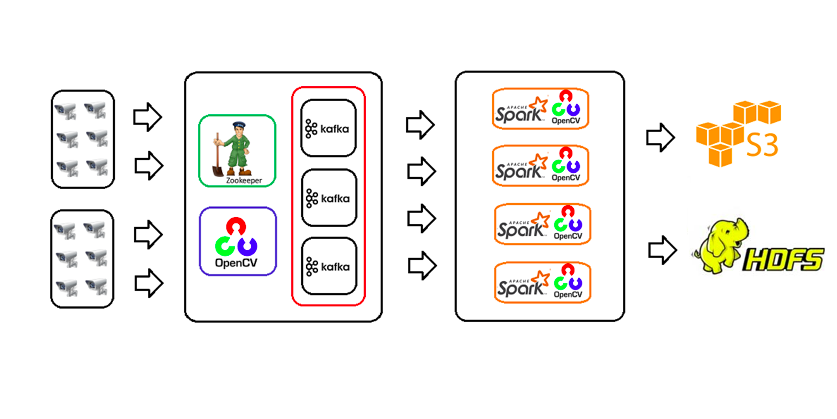
\includegraphics[width=1\textwidth]{amit}
	\caption[Diagrama de la arquitectura presentada por Amit Baghel.]{Diagrama de la arquitectura presentada por Amit Baghel. Fuente: \href{https://www.infoq.com/articles/video-stream-analytics-opencv/}{Infoq}}
\end{figure}

Debido a la similitud de la arquitectura de este trabajo con la que se deseaba contruir se utilizó como base en algunas decisiones del diseño. Concretamente se decidió mantener la configuración planteada para \textit{Kafka}: cantidad de particiones  en tres y el factor de replicación de uno.

Sin embargo, la arquitectura presentada, debido a los cambios de las versiones del los últimos años, ya no se puede desplegar en los sistemas \textit{GNU/Linux} modernos a menos que se compilen directamente las versiones que plantean.